\documentclass{beamer}
\usetheme{metropolis}

% Math packages
\usepackage{amsmath}
\usepackage{amssymb}
\usepackage{amsthm}
\usepackage{mathtools}

\usepackage{tikz}
\usetikzlibrary{automata, positioning, arrows, calc, fit, shapes.misc}

\usepackage{multicol}

\usepackage{todonotes}

\usepackage{subcaption}

% Custom commands
\newcommand{\GFC}{\mathsf{GF}(\mathsf{C})}
\newcommand{\free}[1]{\operatorname{free}(#1)}
\newcommand{\gd}[1]{\operatorname{gd}(#1)}
\newcommand{\RCR}{\operatorname{RCR}}
\newcommand{\CR}{\operatorname{CR}}
\newcommand{\disjunctiveGFC}{\operatorname{disjunctive-\GFC}}
\newcommand{\set}{\operatorname{set}}
\newcommand{\ipo}{i+1\operatorname{mod}}
\newcommand{\Hom}{\operatorname{Hom}}
\newcommand{\C}[1]{\mathsf{C}_{#1}}
\newcommand{\atp}{\operatorname{atp}}
\newcommand{\stp}{\operatorname{stp}}

\renewcommand{\theta}{\vartheta}
\renewcommand{\rho}{\varrho}

\renewcommand{\phi}{\varphi}
\renewcommand{\epsilon}{\varepsilon}

\def\multiset#1{\ensuremath{\left\{\kern-.35em\left\{#1\right\}\kern-.35em\right\}}}
\newcommand{\leftmultiset}{\ensuremath{\{\kern-.35em\{}}
\newcommand{\rightmultiset}{\ensuremath{\}\kern-.35em\}}}


\title{Relational Colour Refinement for Non-Relational Signatures}
\date{September 5, 2025}
\author{Theodor Jurij Teslia}
\institute{RWTH Aachen University}



\begin{document}
	
	\maketitle
	
	\section{Classical Colour Refinement}
	
	\begin{frame}{Colour Refinement}
		\begin{itemize}
			\item Also called CR or $1$-dimensional Weisfeiler-Leman algorithm
			\item Iterative graph algorithm
			\item Constructs colour for every vertex, based on colours of neighbours
		\end{itemize}
		
		\begin{definition}[Colour Refinement]
			For graph $G=(V,E)$, for every $v\in V$ and $i\in \mathbb N$:
			$$C_0(v)\coloneqq 0$$ and $$C_{i+1}(v)\coloneqq(C_i(v),\multiset{C_i(u) : \{v,u\}\in E}).$$
		\end{definition}
	\end{frame}
	
	\begin{frame}{Example for CR}
		\begin{columns}
			\begin{column}{0.25\textwidth}
				\centering
				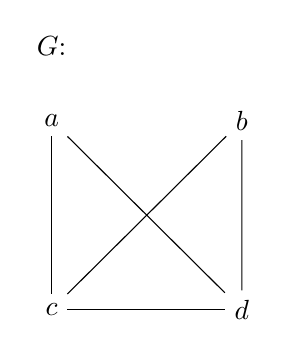
\begin{tikzpicture}[node distance=2cm]
					\node (a) {$a$};
					\node[right=of a] (b) {$b$};
					\node[below=of a] (c) {$c$};
					\node[right=of c] (d) {$d$};
					\node[above=of a, yshift=-1.5cm] (name) {$G$:};
					
					\draw
					(a) edge[-] (c)
						edge[-] (d)
					(b) edge[-] (c)
						edge[-] (d)
					(c) edge[-] (d);
				\end{tikzpicture}
			\end{column}
			\begin{column}{0.75\textwidth}
				\begin{itemize}
					\item $C_0(a)=C_0(b)=C_0(c)=C_0(d)=0$
					\item[]
					\item $C_1(a)=(C_0(a),\multiset{0, 0})=C_1(b)$
					\item $C_1(c)=(C_0(c),\multiset{0, 0, 0})=C_1(d)$
					\item[]
					\item $C_2(a)=(C_1(a),\multiset{C_1(c),C_1(c)})=C_2(b)$
					\item $C_2(c)=(C_1(c),\multiset{C_1(a),C_1(a),C_1(c)})=C_2(d)$
				\end{itemize}
			\end{column}
		\end{columns}
	\end{frame}
	
	\begin{frame}{Distinguished graphs}
		\begin{itemize}
			\item CR distinguishes two graphs $G$ and $H$, if
			\item there exists $C_i(v)$ in colouring of $G$ or $H$, such that number of vertices with colour $C_i(v)$ is different in $G$ than in $H$
		\end{itemize}
		
		\begin{columns}
			\begin{column}{0.25\textwidth}
				\centering
				\begin{tikzpicture}[node distance=2cm]
					\node (a) {$a'$};
					\node[right=of a] (b) {$b'$};
					\node[below=of a] (c) {$c'$};
					\node[right=of c] (d) {$d'$};
					\node[above=of a, yshift=-1.5cm] (name) {$H$:};
					
					\draw
					(a) edge[-] (c)
					edge[-] (d)
					(b) edge[-] (d)
					(c) edge[-] (d);
				\end{tikzpicture}
			\end{column}
			\begin{column}{0.75\textwidth}
				\begin{itemize}
					\item Colours in first round equal
					\item[]
					\item $C_1(b')=(C_0(b'),\multiset{C_0(d')})=(0, \multiset{0})$ does not appear in $G$
				\end{itemize}
			\end{column}
		\end{columns}
		$\Rightarrow$ Colour Refinement distinguishes $G$ and $H$.
	\end{frame}
	
	\begin{frame}{Characterisations of CR}
		\begin{itemize}
			\item There are equivalent characterisations for CR
			\item Due to \textcolor{red}{bibliography}:\break
			CR distinguishes $G$ and $H$ if, and only if, there exists $\phi\in \C{2}$, such that $G\models \phi$ and $H\not\models \phi$
			\item Due to \textcolor{red}{bibliography}:\break
			CR distinguishes $G$ and $H$ if, and only if, there exists tree $T$, such that $\hom(T,G)\neq\hom(T,H)$
		\end{itemize}
		Examples for $G$ and $H$:
		\begin{itemize}
			\item $\phi\coloneqq \exists^{\geq 1} x . \neg \exists^{\geq 2} y . E(x,y)$
			\item $T\coloneqq(\{v, u\}, \{\{v,u\}\})$
		\end{itemize}
	\end{frame}
	
	\section{Relational Colour Refinement}
	
	\begin{frame}{Relational Colour Refinement}
		\begin{itemize}
			\item Introduced by \textcolor{red}{bibliography}
			\item 
		\end{itemize}
	\end{frame}
	
	
\end{document}





















